	%%% LaTeX Template: Article/Thesis/etc. with colored headings and special fonts
%%%
%%% Source: http://www.howtotex.com/

\documentclass[12pt]{article}


\usepackage{apuntes-estilo}
\usepackage{fancyhdr,lastpage}
\usepackage{color,colortbl}
\usepackage{verbatim}

\def\maketitle{

% Titulo 
 \makeatletter
 {\color{bl} \centering \huge \sc \textbf{
  Aplicaciones Multimedia\\ 
\large \vspace*{-8pt} \color{black}Introducción a aplicaciones multimedia. 
 \vspace*{8pt} }\par}
 \makeatother

% Autor
\makeatletter
 {\centering \small 
 	Departamento de Ingeniería de Computadoras \\
 	Facultad de Informática - Universidad Nacional del Comahue \\
 	\vspace{20pt} }
 \makeatother

}

% Custom headers and footers
\fancyhf{} % clear all header and footer fields
\fancypagestyle{plain}{\fancyhf{}}
  	\pagestyle{fancy}
 	\lhead{\footnotesize Aplicaciones multimedia - Departamento de Ingeniería de Computadoras}
 	\rhead{\footnotesize \thepage\ }	% ''Page 1 of 2''

\def\ti#1#2{\texttt{#1} & #2 \\ }



\begin{document}

\thispagestyle{empty}
\maketitle
\setlength{\parindent}{0pt}

\section*{Introducción}

Para comprender el alcance de la palabra multimedia analizaremos distintas 
definiciones. Según la Real Academia Española, multimedia se refiere a un 
adjetivo que indica: ``que utiliza conjunta y simultáneamente diversos 
medios, como imágenes, sonidos y texto, en la transmisión de una 
información.''\cite{raemm}


\begin{figure}[h]
\centering
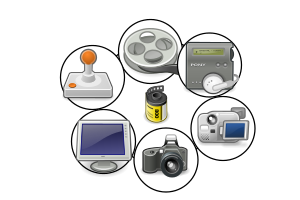
\includegraphics[width=0.8\textwidth]{multimedia.png}
\renewcommand{\figurename}{Fig.}
\caption{https://openclipart.org/detail/201582/multimedia-by-star4clover-201582}
\label{contexto:figura}
\end{figure}

Desde un punto de vista etimológico podemos decir que multimedia se 
refiere a: multi y media. En este sentido ``multi'' se refiere a  muchos, y ``media'' a la
sustancia intermedia a través de la cual algo es transmitido o 
transportado; esto podría ser un medio de comunicación masivo, tal como un periódico o 
la televisión.\cite{ramyer}

Estas definiciones nos dan un primer acercamiento al alcance de la palabra
multimedia. Sin embargo, si nos preguntamos qué aspectos de este alcance 
serían importantes cubrir desde el punto de vista de {\it aplicaciones 
multimediales}, o desde la realidad de un administrador de sistemas y un 
entorno de trabajo convencional, como puede ser una oficina, todavía queda
mucho por aclarar. 

En este sentido la definición de Franklin Kuo, establece dos aspectos del
concepto de multimedia en los cuales haremos foco:

\begin{itemize}
\item Multimedia se refiere a la representación de medios mixtos de información
-texto, datos, imágenes, audio y video- como señales digitales. 
\item Comunicaciones multimedia, se refiere a la tecnología requerida para 
manipular, transmitir y controlar estas señales audiovisuales a través de un 
canal de comunicación.\cite{frankuo}
\end{itemize}


Teniendo los dos aspectos mencionados por Kuo, si nos concentramos en contenidos 
multimedia dentro de una computadora aislada, es decir, sin conexión a red (ya sea LAN o 
Internet), entonces nos enfocaremos por un lado en la representación y almacenamiento 
de datos multimediales, utilizando para ello los conocimientos previos 
adquiridos sobre formato interno de archivos regulares y por otro lado, en 
las {\it aplicaciones multimedia} que nos permiten {\it generar} y manipular 
dichos contenidos localmente. 

Sin embargo, dado la expansión de Internet, y el frecuente desarrollo 
de redes de área local (LAN), debemos dar consideración al segundo aspecto mencionado
por Kuo referente a las {\it Comunicaciones multimediales}. La transmisión 
de datos multimediales sin dudas representa un desafío para los administradores
de sistemas en cuánto al análisis de recursos utilizados en dicha transmisión.
Una transmisión de video en vivo que no llega a tiempo a sus destinos, será 
una comunicación multimedial no exitosa, por lo que el análisis de los 
recursos necesarios se vuelve una tarea compleja e imprescindible en los 
sistemas modernos. 

Por último y no menos importante, abordaremos brevemente los aspectos legales 
sobre la generación y transmisión de contenidos multimedia. En muchos casos,
hemos naturalizado el uso de imágenes, sonidos, textos y videos obtenidos 
desde Internet, sin prácticamente cuestionarnos acerca de la validez 
legal del uso que hacemos. Quizá es más evidente cuando se trata de 
películas o audio, ya que existen multiplicidad de campañas que, mal o 
bien, intentan introducir las consideraciones legales acerca de la descarga y 
reproducción de estos contenidos. Sin embargo, cuántos de nosotros nos 
preguntamos, por ejemplo al desarrollar el contenido de una wiki, si la 
imagen que acabamos de incorporar puede ocasionar un problema legal. 

En resumen, abordaremos multimedia siguiendo tres pilares:
\begin{itemize}
\item Aspectos estáticos: creación, reproducción (aplicaciones y formatos) y 
consumo de recursos, como ser almacenamiento y requisitos de procesamiento. 
\item Aspectos dinámicos: transmisión dentro de redes de área local (LAN) e 
Internet. 
\item Aspectos legales.  
\end{itemize}

\section*{Usos}

Los diferentes formatos de multimedia analógica o digital tienen la 
intención de mejorar la experiencia de los usuarios, por ejemplo para 
que la comunicación de la información sea más fácil y rápida, o, en 
el entretenimiento y el arte, para trascender la experiencia común.\cite{wikipmmes} 

Los usos de la multimedia digital son potencialmente ilimitados. Algunos 
ejemplos de uso que podríamos mencionar son:  

\begin{itemize}
\item {\bf Uso comercial}: publicidad, artistas que distribuyen sus obras como contenidos 
multimediales digitales, venta de productos a través de catálogos en la web, capacitaciones online. 
\item {\bf Entretenimiento y bellas artes}: nuevos desarrollos artísticos y nuevas formas 
de presentación del arte existente, como las galerías de arte online (Google Art Project, 
Museo del Prado, etc) han cobrado vida en los últimos años.  
\item {\bf Educación}: PEDCO podría ser un ejemplo, enciclopedias interactivas, entrenamientos
interactivos, etc. 
\item {\bf Periodismo}: La explosión de los periódicos digitales, la incorporación de dispositivos 
multimediales en los noticieros televisivos, son algunos ejemplos. 
\item {\bf Ingenierías, arquitectura, ciencias en general, medicina}: todas las ciencias se ven 
beneficiadas por el uso de multimedia. La simulación y el modelado son un recurso 
valioso en todas estas áreas del conocimiento. 
\end{itemize}


\section*{Categorizaciones}

Desarrollaremos brevemente dos categorizaciones, ambas relacionadas a la 
percepción del usuario con respecto al contenido multimedia. En un caso 
nos referiremos a la interactividad del usuario, mientras que en el otro 
haremos referencia al componente temporal que puede o no afectar a la
reproducción de los contenidos. 

A la hora de evaluar contenidos multimedia, tendremos en cuenta entonces
por un lado los mecanismos de interacción (si los hubiere), y por otro 
cómo afecta el tiempo a la reproducción de elementos individuales. 

\subsection*{Interactividad}
En cuanto a la interacción que tiene el usuario con un contenido 
multimedial (como un todo, es decir un conjunto de elementos individuales
como texto, imagen, etc), podemos dividir dichos contenidos en: 
\begin{itemize}
\item Lineal: la reproducción de este tipo de contenidos progresa 
sin intervención del observador. Por ejemplo, una presentación cinematográfica.  
\item No lineal: en este caso, la interactividad es utilizada para 
controlar el progreso de la reproducción del contenido multimedial. Por 
ejemplo un video juego, una enciclopedia virtual en donde el observador
avanza a través de los contenidos que prefiere (ejemplo de hypermedia, 
wikipedia es una implementación posible), etc. 
\end{itemize}

\subsection*{Tipos de medios}
Por otra parte, teniendo en cuenta los elementos individuales que componen un 
contenido multimedia, podemos distinguir dos grandes tipos de medios: 

\begin{itemize}
\item{Estáticos, medio discreto independiente del tiempo}: 
Dentro de esta clase encontramos a las imágenes y gráficos fijos, y texto. La información 
en este medio consiste exclusivamente de una secuencia de elementos individuales 
sin un componente de tiempo.
\item{Dinámicos, medio continuo dependiente del tiempo}: 
Aquí encontramos al sonido, animaciones y video. La información no sólo es 
expresada por su valor individual, sino que también por el momento 
de su ocurrencia.
\end{itemize}

Claramente los medios continuos representarán un mayor desafío para el 
administrador a la hora de la transmisión a través de una red. En este 
sentido también podemos subdividir la clasificación en {\it transmisión
en vivo o grabada}. En ambos casos es posible la interactividad, pero 
la transmisión en vivo impone aún más restricciones y desafíos para 
considerarse exitosa. 

Una aclaración importante acerca de esta clasificación es que la noción 
de {\it dependencia del tiempo} no tiene relación con la representación
del dato, en el sentido de que ambos medios, discreto y continuo, en su 
representación física puede no tener información acerca del componente 
temporal. El aspecto temporal en este caso, es más bien la percepción del 
que escucha u observa.\cite{ramyer}  

\section*{Aplicaciones multimedia}

Podríamos comenzar esta sección realizando una lista de aplicaciones 
libres conocidas para multimedia y hacer una descripción breve de cada
una de ellas. Sin embargo además de caer en la obsolescencia mientras 
leemos este apunte, sería imposible ser exhaustivos. Utilizaremos 
algunas aplicaciones a modo de ejemplo y, que al momento de escribir este 
apunte gozan de cierta popularidad.  

El objetivo será entonces, caracterizar las aplicaciones pensando
siempre en nuestro rol de administradores de sistema y, en particular 
en el asesoramiento que usualmente nos es demandado por los usuarios. No
será nuestro objetivo ahondar en el diseño multimedial, sino obtener 
los conocimientos básicos para poder entender la problemática, sugerir 
posibles soluciones o simplemente ser el punto de partida para un análisis 
más profundo cuando el entorno a administrar así lo demande. 

En cada caso trataremos de identificar: 
\begin{itemize}
\item Funcionalidad: ¿Sirve para producir elementos individuales (discretos o continuos) o 
bien es una herramienta que permite la vinculación y presentación de elementos individuales? 
\item Consumo de recursos. Necesidades de la aplicación con respecto al 
hardware y al sistema operativo. Por ejemplo ciertas aplicaciones para generar 
elementos de animación requieren hardware gráfico específico; otras pueden demandar 
una conexión de red para transmitir el contenido, etc. 
\end{itemize}

\subsection*{Gráficos e imágenes estáticas}

Una problemática frecuente es la necesidad de generar y manipular gráficos e imágenes 
bidimensionales. Por citar algunos de los infinitos requisitos posibles, un usuario 
podría necesitar: 
\begin{itemize}
	\item Editar fotos. El usuario desea retocar una o cientos de imágenes capturadas
	      con alguna cámara digital, o escaneadas. En este caso no sólo debemos pensar en el problema de 
	      encontrar software que le permite realizar la edición, sino que también debemos
	      pensar en el mecanismo que le permita importar las fotos como imágenes digitales
	      dentro de su computadora para su posterior edición.    
	\item Creación de imágenes matriciales e imágenes matriciales multicapa (como las generadas por 
	Adobe Photoshop o Gimp).  
	\item Cambiar el formato de una imagen. Por ejemplo pasar uno o cientos de archivos de 
	un formato PNG a JPG. Además podría requerir asesoramiento de qué formato sería el 
	indicado si tuviese que visualizarlo en otros sistemas operativos. 
	\item Crear un diagrama vectorial. Por ejemplo el usuario desea crear un mapa conceptual, o
	un organigrama jerárquico que represente a la organización en la que trabaja.    
	\item Crear una gráfico vectorial (como caso general de lo anterior). Por ejemplo el 
	usuario podría querer crear un logo para la empresa que pueda visualizarse luego en 
	una página web.  
	\item Tomar una captura de pantalla y editarla para luego incorporarla en una presentación. 
	\item Controlar una cámara digital desde la computadora. 
\end{itemize}

Deberemos tener presente al menos que existen: {\bf{\it imágenes matriciales e imágenes vectoriales}}. 
En este sentido:  

``Una imagen vectorial es una imagen digital formada por objetos geométricos independientes (segmentos, 
polígonos, arcos, etc.), cada uno de ellos definido por distintos atributos matemáticos de forma, de 
posición, de color, etc. Por ejemplo un círculo de color rojo quedaría definido por la posición 
de su centro, su radio, el grosor de línea y su color.

Este formato de imagen es completamente distinto al formato de las imágenes de mapa de bits, también 
llamados imágenes matriciales, que están formados por píxeles. El interés principal de los gráficos 
vectoriales es poder ampliar el tamaño de una imagen a voluntad sin sufrir la pérdida 
de calidad que sufren los mapas de bits. De la misma forma, permiten mover, estirar y 
retorcer imágenes de manera relativamente sencilla.'' \cite{wikiives}

``A las imágenes en mapa de bits se las suele definir por su altura y anchura (en píxeles) y por 
su profundidad de color (en bits por píxel), que determina el número de colores distintos que se 
pueden almacenar en cada punto individual, y por lo tanto, en gran medida, la calidad del color de la imagen.''
\cite{wikiimes}

A esto podemos adicionar la existencia de formatos de imagen mas complejos que involucran las antes mencionadas
como base, como ser XCF de Gimp, o PSD de Adobe Photoshop. 

Analizando un poco el consumo de recursos, en lo que a formatos respecta, en general una 
imagen matricial ocupa mayor espacio de almacenamiento que su equivalente vectorial. En el 
primer caso, el tamaño es proporcional al tamaño de la matriz de píxeles (resolución) y a la
profundidad de color de cada píxel (bits por píxel), mientras que en el segundo caso estamos 
hablando de representaciones matemáticas que no varían con el tamaño visualizado. Si bien puede 
darse el caso opuesto, en que la complejidad de las fórmulas matemáticas descriptivas superen 
la versión de mapa de bits, la percepción general es la primera. 

Pensando en las aplicaciones que manipulan estos formatos, en general, la mayoría demandarán al 
menos: hardware gráfico (vulgarmente una placa de video); 
monitor para visualización; cierta capacidad de procesamiento (CPU) y memoria principal (RAM), ya que 
las aplicaciones gráficas, aún cuando nos referimos a imágenes bidimensionales, suelen consumir bastantes 
recursos. También podríamos necesitar elementos de captura de imágenes: cámaras digitales, escáneres, etc.  
Desde los requisitos del sistema operativo, si bien cierto tipo de procesamiento en masa,
por ejemplo el escalado de cientos de imágenes, podría realizarse sin la necesidad de un
entorno gráfico (por ejemplo utilizando el programa convert), en la mayoría de los casos será una 
necesidad. Por otro lado, será necesario que el sistema operativo cuente con los controladores
apropiados para el correcto funcionamiento del hardware, lo cual no es una tarea trivial en 
el mundo del software libre, ya que muchos fabricantes de placas de video (y podríamos decir de hardware
en general) no proveen controladores libres y por ende, puede que las versiones libres 
disponibles (creadas por la comunidad) no exploten todas las características del hardware en cuestión.  

Algunas aplicaciones libres muy populares que podemos mencionar en esta sección son: 
\begin{itemize}
\item Gimp \url{https://directory.fsf.org/wiki/GIMP}, que permite 
trabajar con mapas de bits, e imágenes multicapa. 
\item Inkscape \url{https://directory.fsf.org/wiki/Inkscape}, 
para imágenes vectoriales. 
\item Dia \url{https://directory.fsf.org/wiki/Dia} y Graphviz 
\url{https://directory.fsf.org/wiki/Graphviz}, para diagramas vectoriales de 
varios tipos (mapas mentales, grafos, redes, etc). 
\item DigiKam \url{https://directory.fsf.org/wiki/DigiKam}, nos permite la descarga y organización de 
imágenes tomadas con cámaras digitales. 
\item El comando {\tt convert} realiza varios tipos de procesamiento
en lote (escalado, conversión de formatos, etc). 
\item Hugin \url{https://directory.fsf.org/wiki/Hugin},  
permite la creación de panorámicas a partir de fotos individuales.  
\item Entangle \url{http://entangle-photo.org/}, que permite controlar una cámara 
digital desde la computadora.
\end{itemize}


\subsection*{Sonido}

El sonido es una onda continua que viaja a través del aire y que es percibida por el 
oído humano debido a los cambios de presión generados por esta onda sobre el mismo. 
La representación digital de esas ondas y los recursos necesarios para almacenar, 
reproducir y manipular estos sonidos serán de interés en esta sección (en inglés ``digitize''). . 

Uno de los aspectos a considerar será la representación digital de estas ondas sonoras.
En sí la resolución de estas ondas es infinita. Deberemos entonces pasar de una 
señal analógica continua a alguna forma de representación discreta, posible de ser  
almacenada numéricamente en una computadora. Este será el proceso de digitalización. 
Por ejemplo al utilizar un grabador de sonido (ej. gnome-sound-recorder) proveniente 
de un micrófono y guardar un archivo con esa información, estamos digitalizando la 
onda sonora analógica proveniente del micrófono. 

Sin entrar en los detalles de muestreo y cuantificación de las ondas analógicas, 
una onda sonora será representada digitalmente por una secuencia 
de muestras tomadas en el tiempo en distintos puntos de la onda. Cada muestra 
tendrá un valor que representa la amplitud de la onda en ese punto del tiempo.
La cantidad de muestras por segundo (unidad Hz) y la cantidad de bits usados 
para la amplitud de onda (cuantificación) determinan la calidad de la 
digitalización. Por ejemplo para un CD de audio estándar se utilizan 44100Hz
(44100 muestras por segundo) con una cuantificación de la amplitud de 16 bits
(65536 posibles valores para la amplitud). 


\begin{figure}[h]
\centering
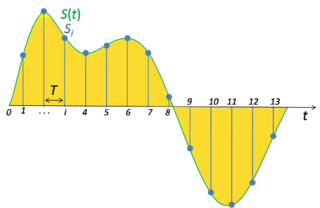
\includegraphics[width=0.8\textwidth]{Sampling.png}
\renewcommand{\figurename}{Fig.}
\caption{http://commons.wikimedia.org/wiki/File:Signal\_Sampling.png}
\label{contexto:figura}
\end{figure}

Una primera deducción que podemos hacer en cuanto al consumo de recursos, y
teniendo en cuenta el muestreo y cuantificación, es que a mayor cantidad de 
muestras por segundo (Hz) y mayor cantidad de bits utilizadas para la
representación de la amplitud, mayor será el tamaño del archivo digital 
generado. A su vez, esto será inversamente proporcional a lo que sucede 
con la calidad de la representación. 

En este sentido, también debemos tener en cuenta que ciertos formatos 
de archivo de audio ocuparán más o menos espacio de almacenamiento, dependiendo 
de estos parámetros y del posible uso de algoritmos de compresión. Por ejemplo 
un archivo con formato {\it wav}\footnote{http://es.wikipedia.org/wiki/Waveform\_Audio\_Format}   
usualmente sin compresión, ocupará mayor espacio de almacenamiento que su
equivalente {\it Ogg Vorbis}\footnote{http://www.vorbis.com/} con 
compresión.

Si quisiéramos ahondar en el tema de sonido y las conversiones, deberíamos 
incluir en nuestro análisis el proceso inverso a la digitalización, por el 
cual un archivo digital de sonido termina produciendo una onda sonora 
analógica. En este aspecto sólo abordaremos las necesidades de hardware
para que esto suceda y las aplicaciones que permiten la reproducción. La
conformación de ondas analógicas a partir de archivos de audio digital 
queda fuera del alcance de este curso. 

Pensemos ahora potenciales requisitos que pueden surgir en cualquier entorno 
de trabajo, relacionados a sonido:
\begin{itemize}
\item Reproducir archivos de audio de distintos tipos y formatos.  
\item Editar un archivo de audio: recortar secciones, 
agregar efectos de sonido, pausas, etc. 
\item Reconocimiento de voz. 
\item Cambios de formato: compresión de audio. 
\item Conferencia de audio. 
\item Controlar la tarjeta de sonido: volumen, efectos, etc.
\item Captura de sonido: micrófono, instrumentos, etc. 
\end{itemize}

Los recursos de hardware necesarios dependerán de estos requisitos.  
En general necesitaremos al menos una tarjeta de sonido que pueda 
recibir y producir señales de audio; las mismas podrán ser integradas
en la placa base o externas, generalmente conectadas a algún bus de
expansión (PCI, PCIE, etc.). Desde el sistema operativo deberemos ser 
capaces de reconocer la presencia de dicho hardware, así como también 
los controladores del sistema operativo adecuados para el efectivo 
funcionamiento del mismo.


\begin{figure}[h]
\centering
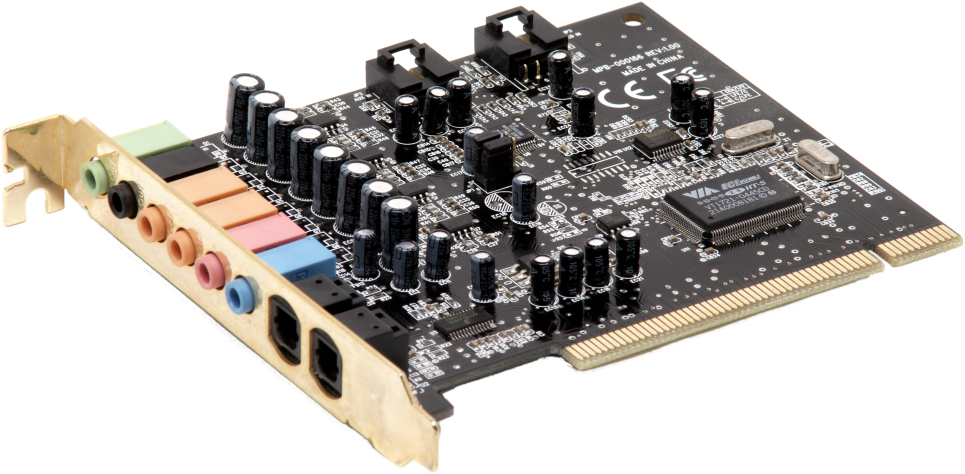
\includegraphics[width=0.8\textwidth]{soundcards.png}
\renewcommand{\figurename}{Fig.}
\caption{http://en.wikipedia.org/wiki/File:Turtle\_Beach\_Sound\_Card\_\%28Catalina\%29.png}
\label{contexto:figura}
\end{figure}

Las tarjetas de sonidos serán las encargadas del proceso de conversión 
analógica/digital y viceversa, para captura/reproducción de audio, explicado 
anteriormente. Adicionalmente, elementos analógicos como ser: parlantes y 
micrófono serán necesarios según el caso. Dicho elementos se conectan 
a la tarjeta de sonido a través de diferentes conectores {\it minijack}.  

En cuanto a {\it aplicaciones libres} que permitan satisfacer diferentes
requisitos relacionados a audio, podemos decir que la mayoría de las distribuciones
ofrecen aplicaciones multimedia para reproducción, mencionaremos algunos 
ejemplos:

\begin{itemize}
\item Rhythmbox \url{https://directory.fsf.org/wiki/Rhythmbox}. GNOME. 
\item Amarok. \url{https://directory.fsf.org/wiki/Amarok}. KDE 
\item Clementine. \url{https://directory.fsf.org/wiki/Clementine}. 
Basado en Amarok. 
\item XMMS. \url{https://directory.fsf.org/wiki/Xmms}. 
\item VLC Media Player. \url{https://directory.fsf.org/wiki/VLC\_media\_player}
Provee interfaz gráfica y en línea de comandos. 
\item Mplayer. \url{http://www.mplayerhq.hu/}. Principalmente utilizado 
desde el intérprete de comandos, sin embargo existen interfaces gráficas
(GUI) como {\it gmplayer} para utilizarlo. 
\end{itemize}

Las últimas dos aplicaciones, son más versátiles en cuánto a los formatos soportados, 
también reproducen video y son {\it independientes del entorno gráfico}, sin embargo 
su interfaz suele ser menos intuitiva que las primeras cuatro aplicaciones 
mencionadas. 
 
Del mismo modo, existen muchas aplicaciones para controlar el nivel del sonido, micrófono, 
líneas de entrada, etc. Normalmente estarán asociadas al entorno gráfico, es decir suelen ser
un componente de software parte de éste. Sin embargo existen algunas independientes como por ejemplo:
{\tt alsamixer}. Será tarea del administrador identificar dicho software dependiendo 
del entorno utilizado por el usuario. 

Las imágenes a continuación se observan dos ejemplos clásicos de aplicaciones provistas
como parte de entornos gráficos: {\it gnome-sound-recorder} que permite la 
digitalización del sonido recibido desde un micrófono o dispositivo de 
entrada conectado a la tarjeta de sonido; esta aplicación es desarrollada como 
parte del entorno gráfico GNOME; la segunda imagen corresponde a la aplicación 
{\it xfce-mixer} perteneciente al entorno gráfico XFCE, que permite controlar 
distintos parámetros como el volumen de salida de la tarjeta de sonido. 


\begin{figure}[h]
\centering
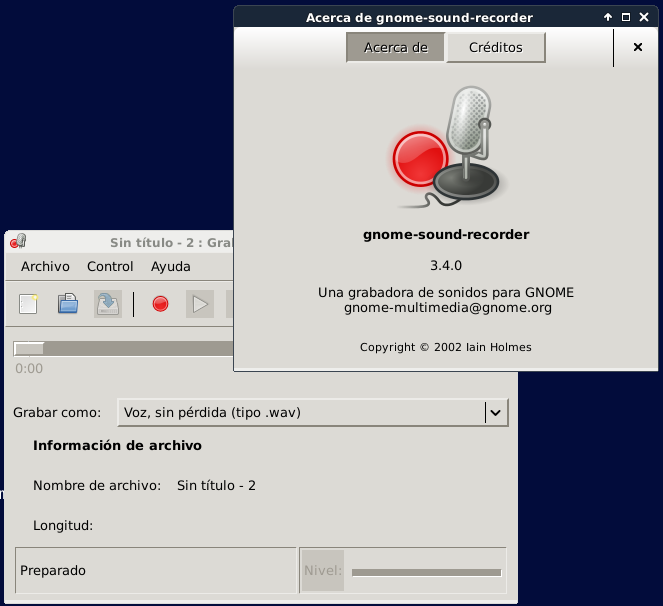
\includegraphics[width=0.8\textwidth]{gnomerec.png}
\renewcommand{\figurename}{Fig.}
\caption{Gnome Sound Recorder}
\label{contexto:figura}
\end{figure}


\begin{figure}[h]
\centering
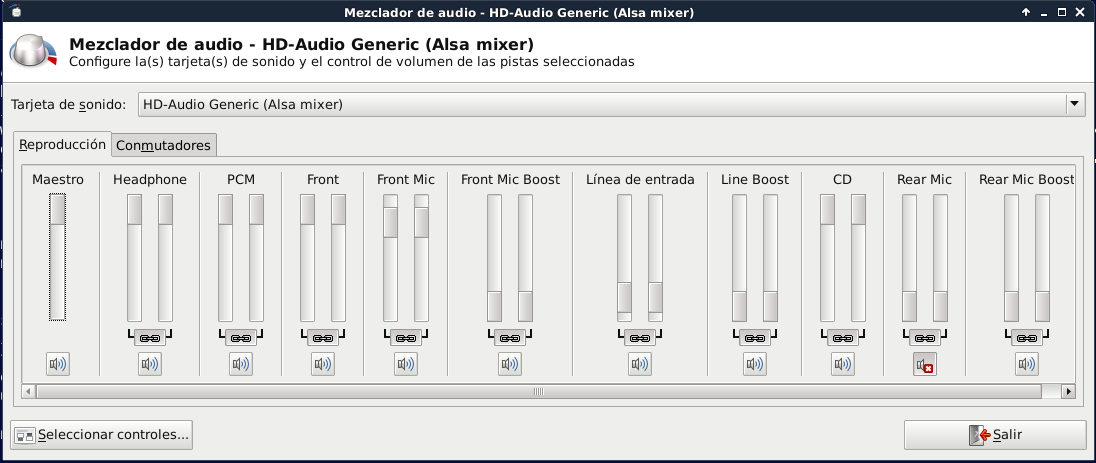
\includegraphics[width=0.8\textwidth]{xfcemix.png}
\renewcommand{\figurename}{Fig.}
\caption{XFCE Mixer}
\label{contexto:figura}
\end{figure}

En cuanto a la dependencia del entorno gráfico, es bueno tener en cuenta que 
la misma se establece a nivel de las bibliotecas compartidas, utilizadas
por la aplicación. Entonces, por ejemplo, si estamos utilizando el entorno gráfico 
GNOME y queremos instalar y ejecutar una aplicación que está diseñada para 
ejecutarse en, digamos, KDE, es muy probable que tengamos que instalar 
bibliotecas del entorno KDE y las mismas serán además ejecutadas adicionalmente 
a las utilizadas por GNOME. En este sentido el administrador de sistemas deberá 
inclinarse por sugerir aplicaciones que, o bien sean independientes, o bien 
utilicen bibliotecas ya instaladas, con el fin de minimizar el consumo de 
recursos. 

Si bien la reproducción y control de audio suelen ser los 
requisitos más comunes de los usuarios, podrían surgir requisitos 
más complejos. Mencionamos algunas aplicaciones y su funcionalidad, 
para dar algunos ejemplos: 

\begin{itemize}
\item Audacity \url{https://directory.fsf.org/wiki/Audacity}.  
Permite la grabación y edición de audio. Por ejemplo (contando con el 
hardware adecuado), podríamos utilizarlo para digitalizar audio proveniente
de casetes, o vinilos. Permite importar archivos en distintos formatos (WAV, 
AIFF, AU, FLAC, OGG Vorbis, MP3, etc) y combinarlos, editarlos, convertir a otros 
formatos, etc. También permite varios tipos de edición: eliminar porciones del 
audio, agregar efectos, eliminar ruido, voces, ajustar volumen. También permite 
el análisis de frecuencias mediante espectrogramas. Por mencionar algunas 
de las posibilidades de este software.  
\item LMMS \url{https://directory.fsf.org/wiki/Linux\Multimedia\studio}.
LMMS es un software libre multiplataforma que permite producir música con 
la computadora. Esto cubre la creación de melodías y ritmos, sintetizar 
y mezclar sonidos y organizar muestras, entre otras características. 
\item Qsynth \url{http://qsynth.sourceforge.net/qsynth-index.html}
Es una interfaz gráfica para la aplicación {\it fluidsynth}, que 
implementa un sintetizador\footnote{Software que emula el funcionamiento 
y sonido que producían los antiguos sintetizadores, además de producir 
más modernos y mejores sonidos.} de tiempo real. 
\item Ardour \url{https://directory.fsf.org/wiki/Ardour}. 
Es un grabador de audio multipista / multicanal profesional y DAW. 
{\it Una estación de trabajo de audio digital (EAD) o DAW por sus siglas 
en inglés (Digital Audio Workstation) es un sistema electrónico dedicado
a la grabación y edición de audio digital por medio de un software de 
edición de audio; y del hardware compuesto por una computadora y una 
interfaz de audio digital, encargada de realizar la conversión 
analógica-digital y digital-analógico dentro de la estación}\cite{wikidawes}.
\item libav (avconv). \url{https://libav.org/}. Proporciona herramientas 
multiplataforma y bibliotecas para convertir, manipular y transmitir 
una amplia gama de formatos multimedia y protocolos. En particular 
{\it avconv} es una de estas herramientas, de línea de comandos (CLI), 
que permite distinto tipo de conversiones de audio y video, incluso 
de una entrada en vivo. También puede convertir entre frecuencias de
muestreo arbitrarias y cambiar el tamaño de vídeo sobre la marcha 
con un filtro polifásico de alta calidad. 
\end{itemize}

Todas las aplicaciones anteriores están orientadas a la edición, conversión 
y producción de audio. Pensando en la manipulación de elementos individuales
que posteriormente formarán (o no) parte de un contenido multimedial más 
complejo. Sin embargo, también existen cientos de posibles requisitos adicionales.
Por ejemplo, los usuarios podrían requerir un sistema de chat de voz como 
el provisto por la aplicación Mumble \url{https://directory.fsf.org/wiki/Mumble}. 
Este tipo de requisitos requieren, además de las cuestiones relativas a la calidad
y el formato, el análisis de los requisitos de transmisión de audio: ancho de banda 
requerido, tipo de red, compresión, etc. 

\subsection*{Video y animación}
Animación: Tupí, Stopmotion (http://linuxstopmotion.org), Blender, 

\begin{itemize}
\item Totem.  \url{https://directory.fsf.org/wiki/Totem}
\end{itemize}

\subsection*{Juntando todo (Authoring)}
Wiki
Openmeeting
Blackboard
Webex
Ofimática: textos, presentaciones, etc. 

\section*{Transmisión}

Calidad del audio vs. tasa de datos (página 152)


\begin{thebibliography}{1}

\bibitem{raemm}
Real Academia Española, \emph{Multimedia}.\hskip 1em plus
0.5em minus 0.4em\url{http://lema.rae.es/drae/?val=multimedia}

\bibitem{ramyer}
Ramesh Yerraballi, \emph{Multimedia Systems, Concepts Standards and 
Practice}.\hskip 1em plus  0.5em minus 0.4em
\url{http://users.ece.utexas.edu/~ryerraballi/MSB/Contents.html}

\bibitem{frankuo}
Franklin F. Kuo, J. Joaquin Garcia Luna-Aceves y Wolfgang Effelsberg. 
\emph{Multimedia Communications: Protocols and Applications}.\hskip 1em plus
  0.5em minus 0.4em\relax Publisher: Prentice Hall; ISBN-13: 978-0138569235  

\bibitem{wikipmmes}
Wikipedia en español. \emph{Multimedia}.\hskip 1em plus
  0.5em minus 0.4em\url{http://es.wikipedia.org/wiki/Multimedia}

\bibitem{wikipmmen}
Wikipedia en inglés. \emph{Multimedia}.\hskip 1em plus
  0.5em minus 0.4em\url{http://es.wikipedia.org/wiki/Multimedia}

\bibitem{wikiives}
Wikipedia en español. \emph{Gráfico Vectorial}.\hskip 1em plus
  0.5em minus 0.4em\url{http://es.wikipedia.org/wiki/Gráfico\_vectorial}

\bibitem{wikiimes}
Wikipedia en español. \emph{Imagen de mapa de bits}.\hskip 1em plus
  0.5em minus 0.4em\url{http://es.wikipedia.org/wiki/Imagen\_de\_mapa\_de\_bits}

\bibitem{wikidawes}
Wikipedia en español. \emph{Estación de trabajo de audio digital}.\hskip 1em plus
  0.5em minus 0.4em\url{http://es.wikipedia.org/wiki/Estaci\%C3\%B3n\_de\_trabajo\_de\_audio\_digital}


\end{thebibliography}{1}

\section*{Licencia}
Copyright (C) 2014 Lechner Miriam.

Se concede autorización para copiar, distribuir y/o modificar este documento
bajo los términos de la Licencia Creative Commons Atribución-CompartirDerivadasIgual 3.0 Unported. 

http://creativecommons.org/licenses/by-sa/3.0/

\end{document}

\end{thebibliography}{1}

\section*{Licencia}
Copyright (C) 2014 Lechner Miriam.

Se concede autorización para copiar, distribuir y/o modificar este documento
bajo los términos de la Licencia Creative Commons Atribución-CompartirDerivadasIgual 3.0 Unported. 

http://creativecommons.org/licenses/by-sa/3.0/

\end{document}
